\section{}
\[
H(s)=\frac{-1000\,(s+2)^2}{4\,(s+1)^3\,(s+10)}=-250\,\frac{(s+2)^2}{(s+1)^3\,(s+10)}\,.
\]
\subsection{Bode-Diagramm}
\begin{center}
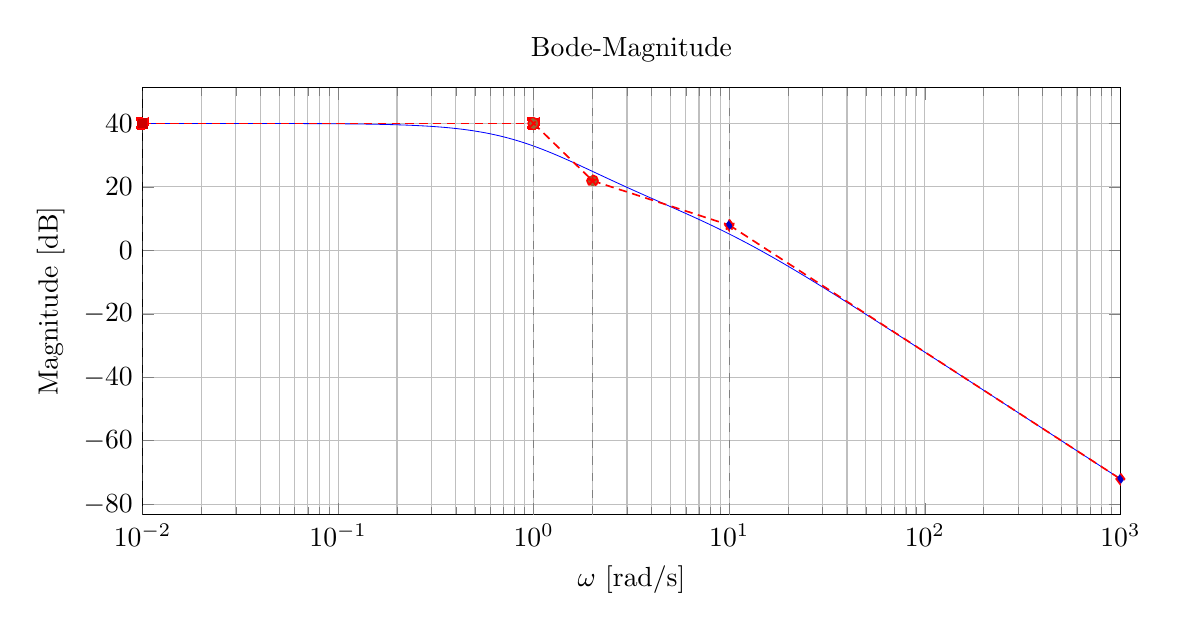
\begin{tikzpicture}
\begin{semilogxaxis}[
  width=14cm,height=7cm,
  ytick distance=20,
  xmin=1e-2,xmax=1e3,
  xlabel={$\omega$ [rad/s]},
  ylabel={Magnitude [dB]},
  grid=both,
  title={Bode-Magnitude}
]
\addplot[
  domain=1e-2:1e3,
  samples=900,
  mark=none,
  line width=0.3pt,
  blue
] {20*ln(250)/ln(10)
    +40*ln(sqrt(4 + x^2))/ln(10)
    -60*ln(sqrt(1 + x^2))/ln(10)
    -20*ln(sqrt(100 + x^2))/ln(10)};
\addplot+[domain=1e-2:1,samples=2,dashed,dash pattern=on 3pt off 2pt,line width=0.6pt,red] {40};
\addplot+[domain=1:2,samples=2,dashed,dash pattern=on 3pt off 2pt,line width=0.6pt,red] {40 - 60*ln(x)/ln(10)};
\addplot+[domain=2:1e1,samples=2,dashed,dash pattern=on 3pt off 2pt,line width=0.6pt,red] {40 - 60*ln(2)/ln(10) - 20*ln(x/2)/ln(10)};
\addplot+[domain=1e1:1e3,samples=2,dashed,dash pattern=on 3pt off 2pt,line width=0.6pt,red] {40 - 60*ln(2)/ln(10) - 20*ln(10/2)/ln(10) - 40*ln(x/10)/ln(10)};
\draw[gray,dashed] (rel axis cs:0,0) -- (rel axis cs:0,1);
\draw[gray,dashed] (axis cs:1,\pgfkeysvalueof{/pgfplots/ymin}) -- (axis cs:1,\pgfkeysvalueof{/pgfplots/ymax});
\draw[gray,dashed] (axis cs:2,\pgfkeysvalueof{/pgfplots/ymin}) -- (axis cs:2,\pgfkeysvalueof{/pgfplots/ymax});
\draw[gray,dashed] (axis cs:10,\pgfkeysvalueof{/pgfplots/ymin}) -- (axis cs:10,\pgfkeysvalueof{/pgfplots/ymax});
\node[gray,anchor=south east] at (axis cs:2,\pgfkeysvalueof{/pgfplots/ymax}) {\scriptsize Nullstelle $\omega_z=2$ (doppelt)};
\node[gray,anchor=south east] at (axis cs:1,\pgfkeysvalueof{/pgfplots/ymax}) {\scriptsize Pol $\omega_p=1$ (dreifach)};
\node[gray,anchor=south east] at (axis cs:10,\pgfkeysvalueof{/pgfplots/ymax}) {\scriptsize Pol $\omega_p=10$};
\end{semilogxaxis}
\end{tikzpicture}
\vspace{6mm}
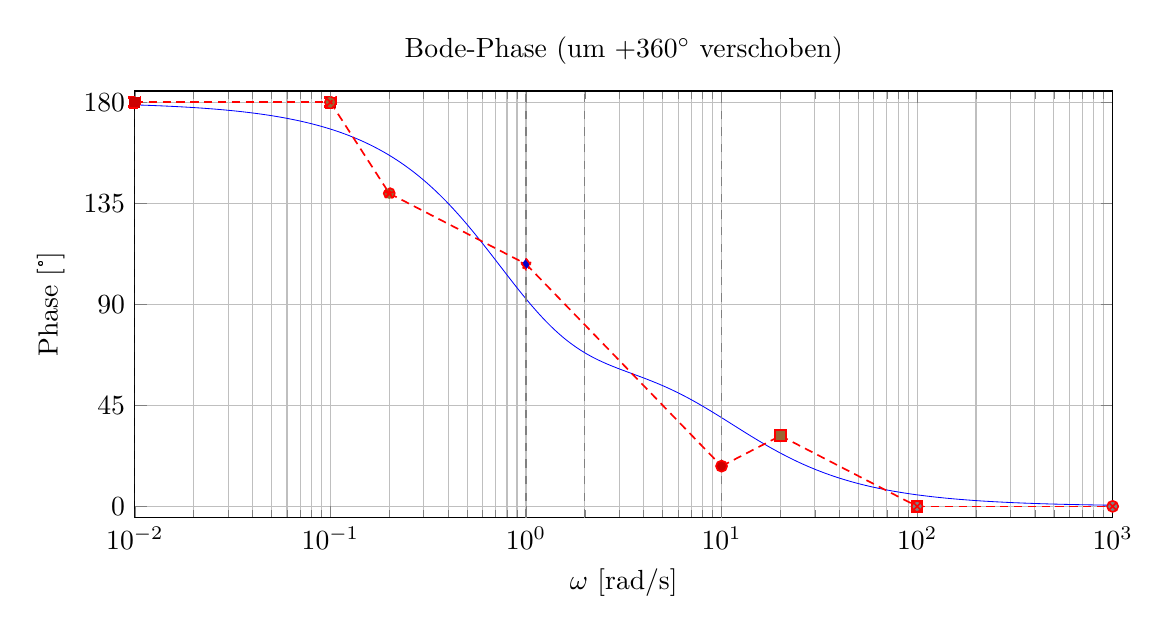
\begin{tikzpicture}
\begin{semilogxaxis}[
  width=14cm,height=7cm,
  xmin=1e-2,xmax=1e3,
  ymin=-5,ymax=185,
  ytick distance=45,
  xlabel={$\omega$ [rad/s]},
  ylabel={Phase [°]},
  grid=both,
  title={Bode-Phase (um $+360^\circ$ verschoben)}
]
% exakte (blaue) Phase: +360° Shift
\addplot[
  domain=1e-2:1e3,
  samples=900,
  mark=none,
  line width=0.3pt,
  blue
] {180 + 2*atan(x/2) - 3*atan(x) - atan(x/10)};

% rote Geradennäherung, korrekt platziert und +360° verschoben
\addplot+[domain=1e-2:1e-1,samples=2,dashed,dash pattern=on 3pt off 2pt,line width=0.6pt,red]{180};
\addplot+[domain=1e-1:2e-1,samples=2,dashed,dash pattern=on 3pt off 2pt,line width=0.6pt,red]{180 - 135*ln(x/0.1)/ln(10)};
\addplot+[domain=2e-1:1e0,samples=2,dashed,dash pattern=on 3pt off 2pt,line width=0.6pt,red]{180 - 135*ln(2)/ln(10) - 45*ln(x/0.2)/ln(10)};
\addplot+[domain=1e0:1e1,samples=2,dashed,dash pattern=on 3pt off 2pt,line width=0.6pt,red]{180 - 135*ln(2)/ln(10) - 45*ln(5)/ln(10) - 90*ln(x)/ln(10)};
\addplot+[domain=1e1:2e1,samples=2,dashed,dash pattern=on 3pt off 2pt,line width=0.6pt,red]{180 - 135*ln(2)/ln(10) - 45*ln(5)/ln(10) - 90 + 45*ln(x/10)/ln(10)};
\addplot+[domain=2e1:1e2,samples=2,dashed,dash pattern=on 3pt off 2pt,line width=0.6pt,red]{180 - 135*ln(2)/ln(10) - 45*ln(5)/ln(10) - 90 + 45*ln(2)/ln(10) - 45*ln(x/20)/ln(10)};
\addplot+[domain=1e2:1e3,samples=2,dashed,dash pattern=on 3pt off 2pt,line width=0.6pt,red]{0};

\draw[gray,dashed] (rel axis cs:0,0) -- (rel axis cs:0,1);
\draw[gray,dashed] (axis cs:1,\pgfkeysvalueof{/pgfplots/ymin}) -- (axis cs:1,\pgfkeysvalueof{/pgfplots/ymax});
\draw[gray,dashed] (axis cs:2,\pgfkeysvalueof{/pgfplots/ymin}) -- (axis cs:2,\pgfkeysvalueof{/pgfplots/ymax});
\draw[gray,dashed] (axis cs:10,\pgfkeysvalueof{/pgfplots/ymin}) -- (axis cs:10,\pgfkeysvalueof{/pgfplots/ymax});
\node[gray,anchor=south east] at (axis cs:2,\pgfkeysvalueof{/pgfplots/ymax}) {\scriptsize Nullstelle $\omega_z=2$ (doppelt)};
\node[gray,anchor=south east] at (axis cs:1,\pgfkeysvalueof{/pgfplots/ymax}) {\scriptsize Pol $\omega_p=1$ (dreifach)};
\node[gray,anchor=south east] at (axis cs:10,\pgfkeysvalueof{/pgfplots/ymax}) {\scriptsize Pol $\omega_p=10$};
\end{semilogxaxis}
\end{tikzpicture}
\end{center}
\newpage

\subsection{Erklärung (ausführlich)}
\begin{description}[leftmargin=1.2em,labelsep=.6em,font=\bfseries]

\item[1. Normalform herstellen.]
\[
H(s)=-250\,\frac{(1+sT_{z})^{2}}{(1+sT_{p1})^{3}\,(1+sT_{p2})},
\quad T_{z}=\tfrac{1}{2},\ T_{p1}=1,\ T_{p2}=\tfrac{1}{10}.
\]
Konstanten:
\[
K_0=-250,\quad r=0.
\]
Einzelteile der Übertragungsfunktion: Doppelnullstelle (LHP) bei \(\omega_z=2\), Dreifachpol (LHP) bei \(\omega_{p1}=1\), einfacher Pol (LHP) bei \(\omega_{p2}=10\).

\item[2. Eckfrequenzen bestimmen und sortieren.]
\[
\omega_{p1}=1\ \text{rad/s}<\omega_{z}=2\ \text{rad/s}<\omega_{p2}=10\ \text{rad/s}.
\]

\item[3. Startpunkt des Amplitudengangs festlegen (Geradennäherung).]
Setze \(\omega_{\min}=\omega_{p1}=1\).
\[
F_{\mathrm{dB}}(\omega_{\min})
=20\log_{10}\!\big(|K_0\,\underline{F}^*_{\!ges}(0)|\,\omega_{\min}^{\,r}\big)
=20\log_{10}(250/2.5)=40\,\mathrm{dB}.
\]
Ankerpunkt: \(40\,\mathrm{dB}\) bei \(\omega=1\).

\item[4. Verlauf links vom Startpunkt zeichnen.]
Für \(\omega<1\): Anfangssteigung \(r\cdot20=0\,\mathrm{dB/dec}\) \(\Rightarrow\) horizontale Asymptote bei \(40\,\mathrm{dB}\).

\item[5. Steigungswechsel an den Eckfrequenzen eintragen.]
Ab \(\omega=1\): \(3 \cdot (-20\,\mathrm{dB/dec})=-60\,\mathrm{dB/dec}\) (Tripelpol).\\
Ab \(\omega=2\) kommt zusätzlich hinzu: \(2\cdot20\,\mathrm{dB/dec}=+40\,\mathrm{dB/dec}\) (Doppelnull) \(\Rightarrow\) netto \(-20\,\mathrm{dB/dec}\) in \([2,10]\).\\
Ab \(\omega=10\): \(-20\,\mathrm{dB/dec}\) (Pol) \(\Rightarrow\) netto \(-40\,\mathrm{dB/dec}\) für \(\omega\gg10\).
Geradennäherung:
\[
|H(j\omega)|_{\mathrm{dB}}\approx
\begin{cases}
40,& \omega<1,\\
40-60\log_{10}\omega,& 1\le\omega<2,\\
40-60\log_{10}2-20\log_{10}(\omega/2),& 2\le\omega<10,\\
40-60\log_{10}2-20\log_{10}5-40\log_{10}(\omega/10),& \omega\ge 10.
\end{cases}
\]

\item[6. Eckabrundungen korrekt berücksichtigen.]
\(\omega=1\) (Tripelpol): \(-3\cdot 3\,\mathrm{dB}=-9\,\mathrm{dB}\) unter der Geradennäherung.\\
\(\omega=2\) (Doppelnull): \(+2\cdot 3\,\mathrm{dB}=+6\,\mathrm{dB}\) über der Geradennäherung.\\
\(\omega=10\) (einfacher Pol): \(-3\,\mathrm{dB}\) unter der Geradennäherung.

\item[7. Phasenstartwert festlegen.]
Da \(K_0\,\underline{F}^*_{\!ges}(0)<0\) und \(r=0\),
\[
\varphi(0)=-180^\circ + r\cdot 90^\circ=-180^\circ
\]
(Plot um \(+360^\circ\) verschoben \(\Rightarrow\) Start bei \(+180^\circ\)).

\item[8. Phasenänderung durch Nullstellen und Pole eintragen.]
Die Phasenlage ergibt sich als Summe der Beiträge aller Glieder und verläuft über die jeweiligen Übergangsdekaden additiv. 
Zunächst setzt der \emph{Tripelpol} bei $\omega=1$ ein: er liefert insgesamt $-270^\circ$ verteilt über die Dekade $[0.1,10]$, d.\,h.\ in seiner aktiven Zone fällt die Phase mit einer Steigung von $-135^\circ/\mathrm{dec}$ (pro einfachem Pol $-45^\circ/\mathrm{dec}$). 
Bei $\omega=2$ beginnt zusätzlich die \emph{Doppelnullstelle} zu wirken, die über $[0.2,20]$ in Summe $+180^\circ$ beisteuert, also $+90^\circ/\mathrm{dec}$ in ihrer Übergangszone. 
Schließlich senkt der \emph{einfache Pol} bei $\omega=10$ die Phase über $[1,100]$ um weitere $-90^\circ$ (Steigung $-90^\circ/\mathrm{dec}$ in seiner aktiven Dekade). 

\textbf{Überlappung/Addierung:} In den überlappenden Bereichen addieren sich die Steigungen: 
Zwischen $[0.2,1]$ wirken Tripelpol ($-135^\circ/\mathrm{dec}$) und Doppelnull ($+90^\circ/\mathrm{dec}$) gleichzeitig, sodass netto $-45^\circ/\mathrm{dec}$ entsteht. 
Im Intervall $[2,10]$ überlagern sich Tripelpol ($-270^\circ$ gesamt) und Doppelnull ($+180^\circ$ gesamt); die resultierende Steigung ist dort netto $-90^\circ/\mathrm{dec}$. 
Sobald ab $\omega=10$ der zusätzliche Pol aktiv wird, bleibt die Null über $[10,20]$ noch wirksam: $+90^\circ/\mathrm{dec}$ (Null) und $-90^\circ/\mathrm{dec}$ (neuer Pol) heben sich auf, sodass netto $+90^\circ/\mathrm{dec}$ in $[10,20]$ resultiert. 


\item[9. Grenzwerte und Konsistenz prüfen.]
DC: \(|H(0)|=|-250\cdot 4/(1^3\cdot 10)|=100\Rightarrow 40\,\mathrm{dB}\); \(\varphi(0)=-180^\circ\) (gezeigt als \(+180^\circ\)).\\
HF: \(|H(j\omega)|\sim 250\,\frac{\omega^2}{\omega^4}=250/\omega^2\Rightarrow -40\log_{10}(\omega/10)-20\log_{10}5\,\mathrm{dB}\); \(\varphi(\infty)=0^\circ\) (mod \(360^\circ\)).

\end{description}

\subsubsection*{Stückweise Näherungen (für die Skizze)}
\[
|H(j\omega)|_{\mathrm{dB}}\approx
\begin{cases}
40,& \omega\ll 1,\\[2pt]
40-60\log_{10}\omega,& 1\ll\omega\ll 2,\\[2pt]
40-60\log_{10}2-20\log_{10}(\omega/2),& 2\ll\omega\ll 10,\\[2pt]
40-60\log_{10}2-20\log_{10}5-40\log_{10}(\omega/10),& \omega\gg 10,
\end{cases}
\]\[
\varphi(\omega)\approx
\begin{cases}
180^\circ,& \omega\le 0.1,\\[2pt]
180^\circ-135^\circ\log_{10}(\omega/0.1),& 0.1<\omega<0.2,\\[2pt]
180^\circ-135^\circ\log_{10}2-45^\circ\log_{10}(\omega/0.2),& 0.2<\omega<1,\\[2pt]
135^\circ-90^\circ\log_{10}(\omega/2),& 2<\omega<10,\\[2pt]
135^\circ-90^\circ\log_{10}5+90^\circ\log_{10}(\omega/10),& 10<\omega<20,\\[2pt]
0^\circ-90^\circ\log_{10}(\omega/20),& 20<\omega<100,\\[2pt]
0^\circ,& \omega\ge 100.
\end{cases}
\]

\newpage